%%%%%%%%%%%%%%%%%%%%%%%%%%%%%%%%%%%%%%%%%%%%%%%%%%%%%%%%%%
%						 								 PREAMBLE	      				 								  %
%%%%%%%%%%%%%%%%%%%%%%%%%%%%%%%%%%%%%%%%%%%%%%%%%%%%%%%%%%
% -*- coding: utf-8 -*-
\nonstopmode
\documentclass[a4paper,12pt]{article}
\usepackage[polish]{babel}
\usepackage{polski}
\usepackage[T1]{fontenc}
\usepackage{marvosym}
\usepackage{xunicode,xltxtra,url,parskip} 	%other packages for formatting
\usepackage[big]{layaureo} 				%better formatting of the A4 page
\usepackage{supertabular} 				%for Grades
\usepackage{hyperref}
\usepackage{fontspec} 					%for loading fonts
\usepackage{titlesec}					%custom \section
\RequirePackage{color,graphicx}
\usepackage[usenames,dvipsnames]{xcolor}
\definecolor{linkcolour}{rgb}{0,0.2,0.6}
\hypersetup{colorlinks,breaklinks,urlcolor=linkcolour, linkcolor=linkcolour}
\usepackage{enumerate}
\defaultfontfeatures{Mapping=tex-text}
\titleformat{\section}{\Large\scshape\raggedright}{}{0em}{}[\titlerule]
\titlespacing{\section}{0pt}{3pt}{3pt}
\addtolength{\voffset}{-1.3cm}
\hyphenation{im-pre-se}
\usepackage{textpos}
\setlength{\TPHorizModule}{10pt} %controls horizontal movements
\setlength{\TPVertModule}{10pt}  %controls vertical movements
\usepackage{needspace}


%%%%%%%%%%%%%%%%%%%%%%%%%%%%%%%%%%%%%%%%%%%%%%%%%%%%%%%%%%
%													BEGIN DOCUMENT						 							 %
%%%%%%%%%%%%%%%%%%%%%%%%%%%%%%%%%%%%%%%%%%%%%%%%%%%%%%%%%%

\begin{document}
\mbox{}
\par{\centering {\Huge \textsc{CV}}\bigskip\par}

%%%%%%%%%%%%%%%%%%%%%%%%%%%%%%%%%%%%%%%%%%%%%%%%%%%%%%%%%%
%											PERSONAL INFORMATION				 									  %
%%%%%%%%%%%%%%%%%%%%%%%%%%%%%%%%%%%%%%%%%%%%%%%%%%%%%%%%%%
%\begin{samepage}
\section{Personal information}
\begin{textblock}{1}(38,0)
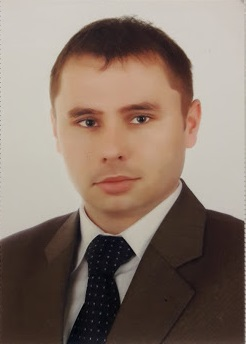
\includegraphics[scale=0.3]{me2.jpg}
\end{textblock}

\begin{tabular}{rl}
	\textsc{First name and surname:}&  \textbf{Robert Ospara} \\
	\textsc{Address:}& Cedrowa 27/95, \\
	\textsc{}& 80-126 Gdańsk, Poland \\
	\textsc{Telephone:}& +48783010280 \\
	\textsc{Email:}& \href{mailto:robertospara@gmail.com}{robertospara@gmail.com}
\end{tabular}

\vspace{2em}

%%%%%%%%%%%%%%%%%%%%%%%%%%%%
%		            TECHNICAL SKILLS       			     
%%%%%%%%%%%%%%%%%%%%%%%%%%%%
\section{Core technical skills and competences}
\begin{tabular}{r|p{9.5cm}}
	\textsc{Web technologies}
	&\footnotesize{JavaScript, CSS, HTML, ASP.NET, ASP.NET MVC, AngularJS, Bootstrap, TypeScript, IIS, Fiddler, SoapUI} \\
	\textsc{Programming Languages}
	&\footnotesize{C\#, C++, C, T-SQL, Perl} \\
	\textsc{Frameworks}
	&\footnotesize{.NET, Entity Framework, SCRUM} \\
	\textsc{Operating Systems}
	&\footnotesize{Microsoft Windows Client and Server} \\
	\textsc{Software Engineering}
	&\footnotesize{OOD, OOP, TDD, UML, architectural and design patterns} \\
	\textsc{Database}
	&\footnotesize{Microsoft SQL Server} \\
	\textsc{IDEs}
	&\footnotesize{Visual Studio, SQL Server Management Studio} \\
\end{tabular}

%%%%%%%%%%%%%%%%%%%%%%%%%%%%%%%%%%%%%%%%%%%%%%%%%%%%%%%%%%
%					FOREIGN LANGUAGES					 %
%%%%%%%%%%%%%%%%%%%%%%%%%%%%%%%%%%%%%%%%%%%%%%%%%%%%%%%%%%
\section{Foreign languages}
\begin{tabular}{r|p{11cm}}
	\textsc{English:}&very good\\
\end{tabular}

%%%%%%%%%%%%%%%%%%%%%%%%%%%%%%%%%%%%%%%
%				WORK EXPERIENCE		  %
%%%%%%%%%%%%%%%%%%%%%%%%%%%%%%%%%%%%%%%
\section{Work experience}
\begin{tabular}{r|p{12cm}}
\textsc{Aug.2013-now}
	&\emph{Software Engineer} \\
	&\textsc{\textbf{Infoprojekt SP. Z O.O.}} (IT) \\
	&\footnotesize{
		Responsibilities: development and maintenance of enterprise software solutions on the stack of Microsoft technologies. \newline
		Current and past activities:
		\begin{itemize}
			\item HelplineDE - development of system for business processes modelling and running.
		        \item Tim -  development of medical factoring system.
		        \item Chronos - development of timetable software linked to the Microsoft TFS.
			\item Helpline - development of tasks scheduling system.
		\end{itemize}
		Used technologies: \newline
		TypeScript 2.X, JS ECMAScript 5, HTML 4.01, HTML5 , Less, CSS3, C\# 6, ASP.NET 4.7.1, Microsoft WebApi 2, AngularJS 1.X, T-SQL,
		OData v3, NServiceBus 6.4.X, EntityFramework 6, Windows Workflow Foundation (WF) , Unity and Moq. \newline
		Used tools: \newline
		Windows Server 2012R2/2016, MSSQL 2012/2014/2016, Visual Studio 2013/2015/2017, TFS 2013/2015/2017.
	}\\
	\multicolumn{2}{c}{}\\

\end{tabular}
%\end{samepage}

\section{Work experience}
\begin{tabular}{r|p{11cm}}
	\textsc{Jun.2012-Jul.2013}
	&\emph{Programmer/Consultant} \\
	&\textsc{\textbf{DC S.A.}} (IT) \\
	&\footnotesize{
		Responsibilities: development and deployment of solutions in Microsoft SharePoint. \newline
		Accomplished projects:
		\begin{itemize}
			\item Documents Organizer - Timer Job that puts in order documents in library in folders of year, quarter and month
			\item Reporting Status Checker - SharePoint's Timer Job that collects statuses of reports from many SPLists and computes some business logic to
												turn
                                             on a proper color of light on dashboard for some business supervisors of this reports; dashboard is a Web Part
			\item Pages Generator - module that generates configurable Web Part Page for meetings when user adds event to SharePoint's calendar;
			architecture is based Publishing Infrastructure
			\item Electronic Card Of New Product - module that generates Content Types for forms of huge workflow in Nitex; second module displays reports
			for workflow's collected data in common application page.
			\item TimeSheet - system that counts working hours and salary of employees
		\end{itemize}
		Used technologies: SharePoint 2010, C\#, ASP.NET, .NET 3.5. Used tools: Windows Server 2008 R2, MSSQL, Visual Studio 2010,
		SVN, Redmine, powershell, SharePoint Designer, SharePoint Manager, InfoPath.
	}\\
	\multicolumn{2}{c}{}\\

	\textsc{Jul.2011-Apr.2012}
	&\emph{Software Development Engineer}\\
	&\textsc{\textbf{Samsung Electronics Polska sp. z o.o.}} (DTV)\\
	&\footnotesize{
		Responsibilities: development of software for DTV platforms; writing tools and tests.\newline
		Accomplished projects:
			\begin{itemize}
				\item Software Upgrade (Search Module) - application for downloading and upgrading DTV's software over the air; I wrote module for
				searching packages of Samsung in ISDB mutex (C++)
				\item Carousel Dumper - tool that takes as input mutex and as output it gives data transmitted in carousel for given parameters (C)
				\item Perforce Efficiency Analyzer - script that updates some files in Perforce (versioning system) permanently each hour and measure
				performance of these actions over the time (Perl)
			\end{itemize}
		Used technologies: C++, C, JavaScript, Perl. Used tools: Linux, Windows XP, Visual Studio, GNU tools, multiplexers,
		stream-players, stream-analyzers, stream-converters, Perforce, Jira.
	}\\
	\multicolumn{2}{c}{}\\



	\textsc{Jun.2010-Jun.2011}
	&\emph{Software Development Engineer}\\
	&\textsc{\textbf{Thomson Reuters (Markets) Europe S.A. Polska}} (finances)\\
	&\footnotesize{ Responsibilities: bugs fixing in the Kondor+. Used technologies: C++.
		Used tools: Solaris, Windows XP, Sybase, Lotus, AquaStudio, SunStudio, SVN.}\\
	\multicolumn{2}{c}{}\\

	\textsc{Nov.2008-May.2009}
	&\emph{C++ Developer}\\
	&\textsc{\textbf{Fluid Desk sp. z o.o.}} (sanitary engineering)\\
	&\footnotesize{Responsibilities: expand utility of XML Library Editor for extensions
		to AUTOCAD. Used technologies: C++, MFC. Used tools: Windows XP, Visual Studio, SVN.}\\
	\multicolumn{2}{c}{}\\
\end{tabular}

\section{Work experience}
\begin{tabular}{r|p{13cm}}
     \textsc{2004-2008}
	&\emph{Software Developer}\\
	&\textsc{\textbf{home (non-commercial)}}\\
	&\footnotesize{Responsibilities: Writing desktop applications, websites, network and client-server solutions for other students.}\\
	\multicolumn{2}{c}{}\\

	\textsc{2002-2006}
	&\emph{Teaching}\\
	&\textsc{\textbf{Mathematics, Physics and Computer Science}}\\
	&\footnotesize{Responsibilities: Helping pupils in maths, physics and computer science.}\\
	\multicolumn{2}{c}{}\\
\end{tabular}

%%%%%%%%%%%%%%%%%%%%%%%%%%%%%%%%%%%%%%%%%%%%%%%%%%%%%%%%%%
%						EDUCATION						 %
%%%%%%%%%%%%%%%%%%%%%%%%%%%%%%%%%%%%%%%%%%%%%%%%%%%%%%%%%%
\section{Education}
\begin{tabular}{r|p{11cm}}
	\textsc{Oct.2006-Nov.2009}
		&  \textbf{Master of Computer Science}\\
	\textsc{Oct.2000-Jun.2003}
		&  \textbf{Nicolaus Copernicus University in Torun Poland}\\
		& Department of Mathematics and Computer Science\\
		& field of study - computer science\\

	\textsc{Sep.1996-Jun.2000}
		& secondary school\\
		& Nicolaus Copernicus High School in Kolobrzeg Poland\\
		& profile of the class - mathematics and physics\\
\end{tabular}


%%%%%%%%%%%%%%%%%%%%%%%%%%%%%%%%%%%%%%%%%%%%%%%%%%%%%%%%%%
%					TRAININGS	    				 	 %
%%%%%%%%%%%%%%%%%%%%%%%%%%%%%%%%%%%%%%%%%%%%%%%%%%%%%%%%%%
\section{Trainings}
\begin{tabular}{r|p{11cm}}
	\textsc{Jul.2014}
	&\emph{Programming in HTML5 with JavaScript and CSS3} \\
	\multicolumn{2}{c}{} \\

	\textsc{Sep.2011}
	&\emph{Microsoft SharePoint 2010 Application Development} \\
	\multicolumn{2}{c}{} \\

	\textsc{Jun.2009-Aug.2009}
	&\emph{Java, C++ Developer} \\
	&\textsc{Tieto Polska sp. z o.o.} (telecommunications) \\
	&\footnotesize{Responsibilities: adding new functionality to network manager. Creating
				   client-server application. Used technologies: C++, Java.} \\
	\multicolumn{2}{c}{} \\

	\textsc{Jul.2006}
	&\emph{Network Administrator} \\
	&\textsc{Wojewodzki Szpital Zespolony im. Ludwika Rydygiera w Toruniu} (public hospital) \\
	&\footnotesize{Responsibilities: solving problems with the hospital network, computers and systems.} \\
	\multicolumn{2}{c}{} \\
\end{tabular}


%%%%%%%%%%%%%%%%%%%%%%%%%%%%%%%%%%%%%%%%%%%%%%%%%%%%%%%%%%
%					SOCIAL WORKS						 %
%%%%%%%%%%%%%%%%%%%%%%%%%%%%%%%%%%%%%%%%%%%%%%%%%%%%%%%%%%
\section{Social works}
\begin{tabular}{r|p{11cm}}
	\textsc{Feb.2011-Jun.2011}
	&\emph{Volunteer}\\
	&\textsc{charity WIOSNA}\\
	&\footnotesize{Responsibilities: helping kids to believe in themselves.}\\
	\multicolumn{2}{c}{}\\

	\textsc{2006-2008}
		&\emph{Volunteer}\\
		&\textsc{orphanage ''Zielony Las'' in Torun}\\
		&\footnotesize{Responsibilities: doing homework with kids.}\\
	\multicolumn{2}{c}{}\\
\end{tabular}


%%%%%%%%%%%%%%%%%%%%%%%%%%%%%%%%%%%%%%%%%%%%%%%%%%%%%%%%%%
%				 ADDITIONAL INFORMATION	     			 %
%%%%%%%%%%%%%%%%%%%%%%%%%%%%%%%%%%%%%%%%%%%%%%%%%%%%%%%%%%
\section{Additional information}
	My hobby is playing basketball, playing guitar, playing chess, reading scientific books and science in general, especially a
	physics of elementary particles, the Standard Model and cosmology. In high school I was a member of basketball
	team in The Province Olympics winning Bronze Medal. I used to represent a sport club SZTORM in running contests.
\vfill{}

\begin{center}
{\scriptsize
	''I hereby give consent for my personal data to be processed for the purposes of recruitment,
	in accordance with the Personal Data Protection Act dated 29.08.1997
	(Journal of Laws of the Republic of Poland 2002 No 101, item 926 with further amendments)''}
\end{center}
\end{document}
